\section{Mechanical analysis}
In this section we will analyze and understand the key dynamics of our robot so we can choose the design parameters based on performance indicators. As parameters we have the with of the flywheel masses $w$, the number of masses $N$, the radius of the flywheel $r_{flywheel}$, and the radius of the wheels $r_{wheel}$

\subsection{Inclination control}
In order to keep the inclination of the platform at a certain angle $\phi$ 
we must be able to compensate all the torque being applied to the platform.

\[\ddot{\phi}\cdot I_{platform} = \tau_{platform} \]

Assuming that the platform is well balanced (the center of masses is located
at the rotation axis by our design restriction) and neglecting the torque generated by the friction
with air, the sum of all the torques in the motor axis applied to the platform
is equal to the sum of the torque applied by the motors:

\[\tau_{platform} = \sum \tau_{motors}\]

The torque that the motors deliver to the wheels and to the flywheel create
a reaction in the platform in the opposite direction.

\[\tau_{platform} = -\tau_{motor-right-wheel} -\tau_{motor-left-wheel} -\tau_{motor-flywheel} \]

If we want keep the inclination $\phi$, we must be able to cancel $\tau_{platform}$.
Observe that the angular acceleration $\ddot{\phi}$ of the platform is linearly 
dependent with the torque it receives. 
\begin{equation} \label{eq:control equation}
\begin{split}
0 = -\tau_{motor-right-wheel} -\tau_{motor-left-wheel} -\tau_{motor-flywheel} \Rightarrow \\
\tau_{motor-right-wheel} +\tau_{motor-left-wheel} = -\tau_{motor-flywheel}
\end{split}
\end{equation}
In other words, we must overpass the torque of the wheels with the torque of the flywheel if we want to control the inclination.

\subsection{Wheels torque}
The wheel torque we can induce is limited by the motor specifications. Note that the maximum torque of the motor is a function of velocity and in particular at max speed the torque is zero.

\[\tau_{motor-wheel} (\omega_{wheel}) \]

\begin{figure}
	\centering
    \begin{tikzpicture}
        %Axis
            \draw[->,thin] (center.center) -- (0,3.5) node[above] {$\tau_{motor}$};
            \draw[->,thin] (center.center) -- (3.5,0) node[right] {$\omega$};
        %Function
            \node (stall) at (0,3) [left]{stall torque};
            \node (maximum) at (3,0) [below]{maximum speed};
            \draw[-] (0,3) -- (3,0);
        \end{tikzpicture}
    \caption{Motor torque}
	\label{fig: Motor torque}
\end{figure}

We assume that the wheels just roll and do no slip.
The robot is pushed by the wheels that make a force $F_{friction}$ against the ground in the contact point. See figure \ref{fig:Wheel force diagram}.

We can express the torque at the center of the of the wheel as:
\[\tau_{motor-wheel} + F_{friction} \cdot r_{wheel} = I_{wheel} 
\cdot \dot{\omega}_{wheel} \]

\begin{equation} \label{wheel torque equation}
\tau_{motor-wheel} = I_{wheel} \cdot \dot{w}_{wheel} - F_{friction} \cdot r_{wheel}
\end{equation}
\begin{figure}[ht]
	\centering
	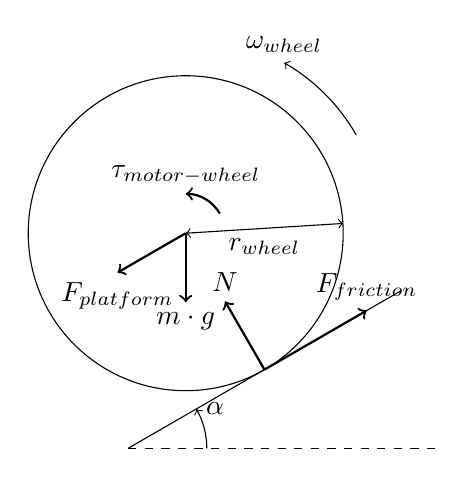
\begin{tikzpicture}
        \path[rotate=30] node (center) at (2,2) {};
        \draw (center) circle (2);
        \draw[rotate=30] (0,0) -- (4,0);
        \draw[dashed] (0,0) -- (4,0);
        \path node[above] (right) at ([shift=({2,0})]center) {};
        \draw[<->] (center.center) -- (right.center)  node[below, midway] {$r_{wheel}$};;
    %Arcs
        \draw[rotate=30, ->] (4.5,2) arc (0:30:2.5) node[above]{$\omega_{wheel}$};
        \draw[rotate=30, ->, thick] (2.5,2) arc (0:60:.5) node[above]{$\tau_{motor-wheel}$};

        \draw[->] (1,0) arc (0:30:1) node[right]{$\alpha$};
    %Forces
        \draw[rotate=30,->,thick] (2,0) -- (3.5,0) node[above]{$F_{friction}$};
        \draw[rotate=30,->,thick] (2,0) -- (2,1) node[above]{$N$};
        \path node[above] (below) at ([shift=({0,-1})]center) {};
    
        \draw[->,thick] (center.center) -- (below.center) node[below]{$m\cdot g$};
        \draw[rotate=30,->,thick] (center.center) -- (1,2) node[below]{$F_{platform}$};
    \end{tikzpicture}
	\caption{Wheel force diagram}
	\label{fig:Wheel force diagram}
\end{figure}


\subsection{Flywheel torque}
\begin{figure}
	\centering
    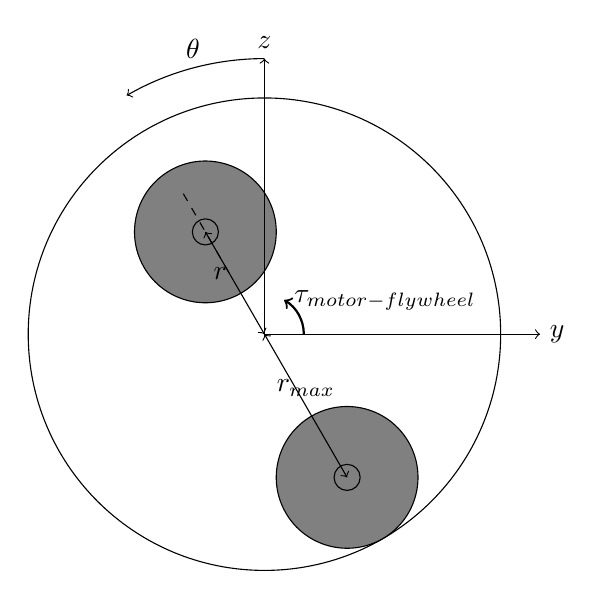
\begin{tikzpicture}
        %Circle
            \path node (center) at (0,0) {};
            \draw (center) circle (3);
        %Arcs
            \draw[->] (0,3.5) arc (90:120:3.5) node[above, midway]{$\theta$};
        %Movable mass
            \draw[rotate=120,fill=gray] (1.5,0) circle (.9) node (moving) [draw,circle]{};
        %Guide
            \draw[dashed,rotate=120] (.9,0) -- (2.1,0);
        %Other masses
            \foreach \i in {2}
            {
                \draw[rotate=60-60* \i,fill=gray] (3-.9,0) circle (.9) node[draw,circle]{};
            }
        %Radius
            \draw[<->] (0,0) -- (moving.center) node[near end, below] {$r$};
            \draw[rotate=-60,<->] (0,0) -- (2.1,0) node[midway, above] {$r_{max}$};
        %Axis
            \draw[->,thin] (center.center) -- (0,3.5) node[above] {$z$};
            \draw[->,thin] (center.center) -- (3.5,0) node[right] {$y$};
        %Motor torque
        \draw[->, thick] (0.5,0) arc (0:60:.5) node[right]{$\tau_{motor-flywheel}$};    
    \end{tikzpicture}
            \caption{Flywheel diagram for $N$ = 2}
	\label{fig:Flywheel force diagram}
\end{figure}

The flywheel torque we can induce is also limited by the motor specifications. 

Assuming a general configuration of the flywheel where the moving mass is at distance $r$ from the axis and angle $\theta$, see figure \ref{fig:Flywheel force diagram}. We formulate its torque the following way:
\[
    \tau_{motor-flywheel} + m_{cylinder} \cdot g \cdot (r - r_{max}) \cdot \sin{\theta} = \ddot{\theta}\cdot I_{flywheel}(r)  
\]
\begin{equation}\label{eq: flywheel torque equation}    
    \tau_{motor-flywheel} = \ddot{\theta}\cdot I_{flywheel}(r) + m_{cylinder} \cdot g \cdot (r_{max} - r) \cdot \sin{\theta}  
\end{equation}

Note that in equation \ref{eq: flywheel torque equation} the two terms correspond to the two methods: accelerating and non vertical position.

\subsection{Maximum speed, acceleration and inclination}
In this subsection we would like to study the maximum speed and acceleration the robot may obtain in straight direction facing and inclination $\alpha$.

We will assume both wheels turn at the same speed, have the same $F_{friction}$ and the same $\tau_{wheel}$:
\[ \omega_{wheel-left} = \omega_{wheel-right} = \omega_{wheel} \]

\begin{figure}
	\centering
	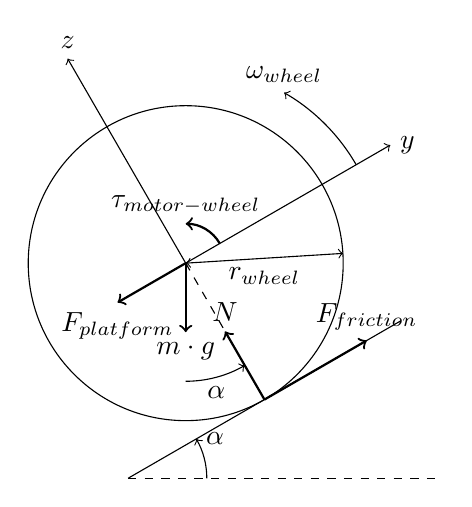
\begin{tikzpicture}
        \path[rotate=30] node (center) at (2,2) {};
        \draw (center) circle (2);
        \draw[rotate=30] (0,0) -- (4,0);
        \draw[dashed] (0,0) -- (4,0);
        \path node[above] (right) at ([shift=({2,0})]center) {};
        \draw[<->] (center.center) -- (right.center)  node[below, midway] {$r_{wheel}$};;
    %Arcs
        \draw[rotate=30, ->] (4.5,2) arc (0:30:2.5) node[above]{$\omega_{wheel}$};
        \draw[rotate=30, ->, thick] (2.5,2) arc (0:60:.5) node[above]{$\tau_{motor-wheel}$};

        \draw[->] (1,0) arc (0:30:1) node[right]{$\alpha$};
        \draw[rotate=30,<-] (2,.5) arc (270:240:1.5) node[below, midway]{$\alpha$};
    %Forces
        \draw[rotate=30,->,thick] (2,0) -- (3.5,0) node[above]{$F_{friction}$};
        \draw[rotate=30,->,thick] (2,0) -- (2,1) node[above]{$N$};
        \path node[above] (below) at ([shift=({0,-1})]center) {};
    
        \draw[->,thick] (center.center) -- (below.center) node[below]{$m\cdot g$};
        \draw[rotate=30,->,thick] (center.center) -- (1,2) node[below]{$F_{platform}$};
    %Axis
        \draw[->,thin][rotate=30] (center.center) -- (2,5) node[above] {$z$};
        \draw[->,thin][rotate=30] (center.center) -- (5,2) node[right] {$y$};
        \draw[dashed][rotate=30] (center.center) -- (2,1);

    \end{tikzpicture}
    \caption{Wheel forward force diagram}
    \label{fig:Wheel forward force diagram}
\end{figure}

Applying Newton's first law in the y axis of figure \ref{fig:Wheel forward force diagram}:
\[\ddot{y}\cdot m_{total} = 2 \cdot F_{friction} - m_{total} \cdot g \cdot sin(\alpha)\]

Substituting $F_{friction}$ taking in to account equation \ref{wheel torque equation}:
\[\ddot{y}\cdot m_{total} = 2 \cdot \frac{I_{wheel} \cdot \dot{w}_{wheel}-\tau_{motor-wheel}}{r_{wheel}} - m_{total} \cdot g \cdot sin(\alpha)\]

Using equation \ref{eq:control equation}:
\begin{equation}\label{eq of acceleration}
    \Rightarrow  \ddot{y}\cdot m_{total} = \frac{2\cdot I_{wheel} \cdot \dot{w}_{wheel}}{r_{wheel}} + \frac{\tau_{motor-flywheel}}{r_{wheel}} - m_{total} \cdot g \cdot sin(\alpha)
\end{equation}


We will now study different cases to better understand this equation.
\subsubsection{No terrain inclination ($\alpha = 0$)}
The objective here is to obtain the maximum speed and acceleration we can get starting from rest in a plain surface.

The equation we get by substituting $\alpha = 0$ in equation \ref{eq of acceleration}:
\[\ddot{y}\cdot m_{total} = \frac{\tau_{motor-flywheel}}{r_{wheel}} +\frac{2\cdot I_{wheel} \cdot  \dot{w}_{wheel}}{r_{wheel}}\]

Substituting equation \ref{eq: flywheel torque equation}:
\begin{equation}\label{eq: no inclintation}
    \ddot{y}\cdot m_{total} = \frac{\ddot{\theta}\cdot I_{flywheel}(r) +
    m_{cylinder} \cdot  g \cdot  (r_{max} - r) \cdot  \sin{\theta}}{r_{wheel}} +\frac{2\cdot I_{wheel} \cdot  \dot{\omega}_{wheel}}{r_{wheel}}
\end{equation}


We will now split the study in two cases:
\begin{enumerate}
    \item Flywheel case: $r$ is fixed to $r = r_{max}$ 
    
    Then:  
    \[\ddot{y}\cdot m_{total} = - \frac{\ddot{\theta}\cdot I_{flywheel}(r_{max})}
    {r_{wheel}} + \frac{2\cdot I_{wheel} \cdot  \dot{\omega}_{wheel}}{r_{wheel}}\]

    Taking in to account the following relation:
    \begin{equation} \label{eq: angular velocity}
        -\omega_{wheel} \cdot  r_{wheel} = \dot{y} \Rightarrow  -\dot{\omega}_{wheel} \cdot  r_{wheel} = \ddot{y}  
    \end{equation}

    Substituting in equation \ref{eq: no inclintation}:
    \[-\dot{\omega}_{wheel} \cdot  r_{wheel}\cdot m_{total} = \frac{\ddot{\theta}\cdot I_{flywheel}}
    {r_{wheel}} + \frac{2\cdot I_{wheel} \cdot  \dot{\omega}_{wheel}}{r_{wheel}} \]

    \[-\dot{\omega}_{wheel} \cdot (r_{wheel}\cdot m_{total} +  \frac{2\cdot I_{wheel} }{r_{wheel}}) = 
    \frac{\ddot{\theta}\cdot I_{flywheel}}{r_{wheel}}\]


    We now define R as a non dimensional constant beeing the the quotient between $\dot{w}_{wheel}$ and $-\ddot{\theta}$.

    \begin{equation}\label{eq: R definition}
        R = \frac{\dot{\omega}_{wheel}}{-\ddot{\theta}} = 
    \frac{I_{flywheel}}
    {r_{wheel}^2\cdot m_{total} +  2\cdot I_{wheel}}
    \end{equation}

    The moments of inertia are:
    \[I_{wheel} \approx \frac{1}{2} \cdot m_{wheel} \cdot  r_{wheel}^2\]
    \[I_{flywheel} \approx N \cdot  m_{cylinder} \cdot  r_{max}^2\]

    Substituting those in equation \ref{eq: R definition} we get:
    \[R \approx
    \frac{ N \cdot  m_{cylinder} \cdot  r_{max}^2}
    {r_{wheel}^2\cdot m_{total} +  2\cdot I_{wheel}} < 1 \] 

    We can see that R will always be smaller than 1 because $N \cdot  m_{cylinder} < m_{total} $ and $r_{max} < r_{wheel}$.
    
    This means that we will the maximum acceleration of the wheels will be limited by the acceleration of the flywheel. The same is true for the speed.

    In  order to get the forward acceleration we can use equation \ref{eq: angular velocity}
    \[\ddot{y} = -\dot{\omega}_{wheel} \cdot  r_{wheel} = R \cdot  \ddot{\theta} \cdot  r_{wheel}\]

    And using equation \ref{eq: flywheel torque equation} we get that the maximum is:

    \[\tau_{motor} (\omega) = \ddot{\theta}\cdot I_{flywheel}(r) \Rightarrow \ddot{\theta} = \frac{\tau_{motor} (\dot{\theta})}{I_{flywheel}(r)} \]

    \[\ddot{y}_{max} = R \cdot  \frac{\tau_{motor} (\dot{\theta})}{I_{flywheel}(r)} \cdot  r_{wheel}\]

    \[\Rightarrow \ddot{y}_{max} =     \frac{I_{flywheel}}
    {r_{wheel}^2\cdot m_{total} +  2\cdot I_{wheel}}  \cdot  \frac{\tau_{motor} (\dot{\theta})}{I_{flywheel}(r)} \cdot  r_{wheel}\]
    \begin{equation}        
        \boxed{\ddot{y}_{max} = \frac{\tau_{motor}(\dot{\theta})\cdot r_{wheel} }
        {r_{wheel}^2\cdot m_{total} +  2\cdot I_{wheel}}}
        \label{maximum acceleration flywheel}
    \end{equation}
    In order to compute the maximum speed we assume that the initial conditions are $\dot{\theta} = 0$ and 
    $\omega_{wheel}=0$

    \[\omega_{wheel-max} = \int_{t=0}^{t=t_{max}} \dot{\omega}_{wheel} \cdot  dt\]

    Now we will proceed to do a change of variables in the integral.

    \[
    \frac{\partial \dot{\theta}}{\partial t} = \ddot{\theta} \Rightarrow dt = \frac{d\dot{\theta}}{\ddot{\theta}}
    \]
    
    \[\omega_{wheel-max} = \int_{\dot{\theta}=0}^{\dot{\theta}=\dot{\theta}_{max}} \frac{\dot{w}_{wheel}}{\ddot{\theta}} \cdot  d\dot{\theta} = 
    \int_{\dot{\theta}=0}^{\dot{\theta}=\dot{\theta}_{max}} -R \cdot  d\dot{\theta} = - R \cdot  \dot{\theta}_{max}
    \]
    \begin{equation}
        \boxed{\dot{y}_{max} = r_{wheel} \cdot  R \cdot  \dot{\theta}_{max}}
        \label{Maximum speed flywheel}
    \end{equation}
    And $\dot{\theta}_{max}$ is a limitation imposed by the motor specifications. Note that this is the maximum speed
    we can get using the flywheel system starting from rest.


    \item Pendulum: $\dot{\theta} = 0$, and $r$ is fixed to $r = r_{min}$
    
    Using equation \ref{eq: no inclintation} and $\ddot{\theta} = 0$
    \[\ddot{y}\cdot m_{total} = \frac{m_{cylinder} \cdot  g \cdot  (r_{max} - r_{min}) \cdot  \sin{\theta}}{r_{wheel}} +\frac{2\cdot I_{wheel} \cdot  \dot{w}_{wheel}}{r_{wheel}}\]
    Multiplying by $r_{wheel}$ both sides of the equation we get:
    \[\ddot{y}\cdot m_{total} \cdot  r_{wheel} = m_{cylinder} \cdot  g \cdot  (r_{max}-r_{min}) \cdot  \sin{\theta} + 2\cdot I_{wheel} \cdot  \dot{w}_{wheel}\]
    And using $\dot{w}_{wheel} = -\frac{\ddot{y}}{r_{wheel}}$
    \[\ddot{y}\cdot m_{total} \cdot  r_{wheel} + 2\cdot  I_{wheel} \cdot  \frac{\ddot{y}}{r_{wheel}} = m_{cylinder} \cdot  g \cdot  (r_{max}-r) \cdot  \sin{\theta} \]
    With some manipulation:
    \[\ddot{y}  = \frac{m_{cylinder} \cdot  g \cdot  (r_{max}-r_{min}) \cdot  \sin{\theta}}{m_{total} \cdot  r_{wheel} + \frac{2\cdot I_{wheel}}{r_{wheel}} }  \]
    Which is maximum when $\sin{\theta}=1$
    \begin{equation}
        \boxed{ \ddot{y}_{max}  = \frac{m_{cylinder} \cdot  g \cdot  (r_{max}-r_{min}) \cdot}{m_{total} \cdot  r_{wheel} + \frac{2\cdot I_{wheel}}{r_{wheel}} } }
        \label{maximum acceleration pendulum}
    \end{equation}
    We need to take into consideration air friction to see the speed limitation in the pendulum case.
    \[F_{drag} = \frac{1}{2}\cdot \rho\cdot C_D \cdot  A \cdot  \dot{y}^2 \]

    Adding this term to equation \ref{eq of acceleration} we get:
    \[  \ddot{y}\cdot m_{total} = \frac{2\cdot I_{wheel} \cdot  \dot{w}_{wheel}}{r_{wheel}} + \frac{\tau_{motor-flywheel}}{r_{wheel}} - m_{total} \cdot  g \cdot  sin(\alpha) - F_{drag} \]
    And making $\ddot{y} = 0$ and $\alpha = 0$.
    \[  F_{drag} = \frac{\tau_{motor-flywheel}}{r_{wheel}}\]

    \[\frac{1}{2}\cdot \rho\cdot C_D \cdot  A \cdot  \dot{y}^2 = m_{cylinder} \cdot  g \cdot  (r_{max} - r_{min})\cdot sin(\theta) / r_{wheel} \]
    The maximum $\dot{y}$ is then obtained when $\theta=\frac{\pi}{2}$:
    \begin{equation*}
        \dot{y}_{max} = \sqrt{\frac{2\cdot m_{cylinder} \cdot  g \cdot  (r_{max} - r_{min})}{\rho\cdot C_D \cdot  A \cdot  r_{wheel}} }
    \end{equation*}

    We will pick $C_D=1$, $\rho=1.2 kg/m^3$ and $A=0.01 m^2$ for our computations.

    Also note that the speed is also limited by maximum speed a motor can get
    $\dot{\theta}_{max}$.
    \begin{equation}
        \boxed{\dot{y}_{max} = min(\dot{\theta}_{max}\cdot r_{wheel}, \sqrt{\frac{2\cdot m_{cylinder} \cdot  g \cdot  (r_{max} - r_{min})}{\rho\cdot C_D \cdot  A \cdot  r_{wheel}} })}
        \label{maximum speed pendulum}
    \end{equation}


\end{enumerate}
\subsubsection{No acceleration, just inclination ($\alpha > 0$)}
The goal of this subsubsection is to study which is the maximum inclination $\alpha_{max}$ the robot can overpass.

Substituting $\ddot{y}=0$ and $\dot{\omega}_{wheel} = 0$ in equation \ref{eq of acceleration}
\[0 = \frac{\tau_{motor-flywheel}}{r_{wheel}} - m_{total} \cdot  g \cdot  sin(\alpha)\]
\[m_{total} \cdot  g \cdot  sin(\alpha) = \frac{\tau_{motor-flywheel}}{r_{wheel}} \]
\[sin(\alpha) = min(1,\frac{\tau_{motor-flywheel}}{m_{total} \cdot  g \cdot  r_{wheel}}) \]

Substituting equation \ref{eq: flywheel torque equation}
\[sin(\alpha) = min(1,\frac{\ddot{\theta}\cdot I_{flywheel}(r) + m_{cylinder} \cdot  g \cdot  (r_{max} - r) \cdot  \sin{\theta}}{m_{total} \cdot  g \cdot  r_{wheel}}) \]


We are going to distinguish the same two cases as in the previous section:
\begin{enumerate}
    \item Flywheel case: $r$ is fixed to $r = r_{max}$
    The maximum inclination at a certain moment:
    \begin{equation}\label{Maximum angle using flywheel system}
        \boxed{sin(\alpha_{max}) = min(1,\frac{\ddot{\theta}\cdot I_{flywheel}}{m_{total} \cdot  g \cdot  r_{wheel}}) = min(1,\frac{\tau_{motor-flywheel}(\dot{\theta})}{m_{total} \cdot  g \cdot  r_{wheel}})}
    \end{equation}


    This angle doesn't give us a lot of information because it may not be fulfilled in a 
    permanent state. That's why in addition we would like to compute the maximum height
    our robot can achieve start from rest position.
    \item Pendulum: $\dot{\theta} = 0$, and $r$ is fixed to $r = r_{min}$
    \[sin(\alpha) = \frac{min(\tau_{motor-flywheel},m_{cylinder} \cdot  g \cdot  (r_{max} - r_{min}) \cdot  \sin{\theta})}{m_{total} \cdot  g \cdot  r_{wheel}} \]
    Which is maximum when $\sin{\theta} = 1$
    \begin{equation}\label{Maximum angle using pendulum system}
        \boxed{sin(\alpha_{max}) = \frac{min(\tau_{motor-flywheel},m_{cylinder} \cdot  g \cdot  (r_{max} - r_{min}))}{m_{total} \cdot  g \cdot  r_{wheel}}}
    \end{equation}
    Note that the $sin(\alpha_{max})$ will not be more than 1.
\end{enumerate}

\subsubsection{Flywheel maximum height}
    \paragraph{Computing $\theta(t)$:} Before we compute the height the robot can obtain using the flywheel system
    we need to define how the flywheel will be turning.
    We will assume that $\tau_{motor-flywheel}$ is always equal to the maximum torque the motor may apply.
    \[\tau_{motor}(\dot{\theta}) \approx \tau_{max}- \dot{\theta}\cdot\frac{\tau_{max}}{\dot{\theta}_{max}}\]
    Using equation \ref{eq: flywheel torque equation}:
    \[\dot{\theta}(t)=\int \ddot{\theta}(t) dt
    = \frac{1}{I_f} \int \tau_{max}- \dot{\theta}(t)\cdot\frac{\tau_{max}}{\dot{\theta}_{max}} dt \]

    \[\dot{\theta}(t) = \frac{\tau_{max}\cdot t}{I_f} - \frac{\tau_{max}}{I_f \cdot \dot{\theta}_{max}}\int \dot{\theta}(t) dt \]
    \[\dot{\theta}(t) + \frac{\tau_{max}}{I_f \cdot \dot{\theta}_{max}}\cdot \theta(t) = \frac{\tau_{max}\cdot t}{I_f} \]
    Which is a non-homogeneous first order differential equation with solution:
    \begin{equation}
        \label{eq: non-homogeneous solution}
        \theta(t) = \frac{\int(\mu(t) \cdot \frac{\tau_{max}\cdot t}{I_f})dt}{\mu(t)}
    \end{equation}
    Being $\mu(t)$:    
    \begin{equation*}
        \mu(t) = e^{\int \frac{\tau_{max}}{I_f \cdot \dot{\theta}_{max}} dt} = e^{t\cdot \frac{\tau_{max}}{I_f \cdot \dot{\theta}_{max}}+C_1}
    \end{equation*}
    Integrating by parts to get the numerator:
    \begin{equation*}
        \int(\mu(t) \cdot \frac{\tau_{max}\cdot t}{I_f})dt = \frac{\tau_{max}\cdot t}{I_f}\cdot\int\mu(t) - \int (\int \mu(t) dt) \cdot \frac{\tau_{max}}{I_f}dt
    \end{equation*}
    \begin{equation*}
        \int \mu(t) dt = \frac{I_f \cdot \dot{\theta}_{max}}{\tau_{max}} \cdot (e^{t\cdot \frac{\tau_{max}}{I_f \cdot \dot{\theta}_{max}}+C_1}+C_2)
    \end{equation*}
    \begin{equation*}
        \dot{\theta}_{max} \cdot t\cdot (e^{t\cdot \frac{\tau_{max}}{I_f \cdot \dot{\theta}_{max}}+C_1}+C_2) - \frac{I_f \cdot \dot{\theta}_{max}^2}{\tau_{max}} \cdot (e^{t\cdot \frac{\tau_{max}}{I_f \cdot \dot{\theta}_{max}}+C_1}+C_2) +C_3
    \end{equation*}
    \begin{equation*}
        (\dot{\theta}_{max} \cdot t- \frac{I_f \cdot \dot{\theta}_{max}^2}{\tau_{max}})\cdot (e^{t\cdot \frac{\tau_{max}}{I_f \cdot \dot{\theta}_{max}}+C_1}+C_2)+C_3 
    \end{equation*}
    Substituting on equation \ref{eq: non-homogeneous solution}:
    \begin{equation*}
        \theta(t) = \frac{(\dot{\theta}_{max} \cdot t- \frac{I_f \cdot \dot{\theta}_{max}^2}{\tau_{max}})\cdot (e^{t\cdot \frac{\tau_{max}}{I_f \cdot \dot{\theta}_{max}}+C_1}+C_2)+C_3 }
        {e^{t\cdot \frac{\tau_{max}}{I_f \cdot \dot{\theta}_{max}}+C_1}}
    \end{equation*}


    \begin{equation*}
        \theta(t) = \frac{(\dot{\theta}_{max} \cdot t- \frac{I_f \cdot \dot{\theta}_{max}^2}{\tau_{max}})\cdot C_2 }
        {e^{t\cdot \frac{\tau_{max}}{I_f \cdot \dot{\theta}_{max}}+C_1}} 
        + (\dot{\theta}_{max} \cdot t- \frac{I_f \cdot \dot{\theta}_{max}^2}{\tau_{max}})
        + \frac{C_3 }
        {e^{t\cdot \frac{\tau_{max}}{I_f \cdot \dot{\theta}_{max}}+C_1}}
    \end{equation*}
Renaming the constants we get:
    \begin{equation*}
        \theta(t) = \frac{(\dot{\theta}_{max} \cdot t- \frac{I_f \cdot \dot{\theta}_{max}^2}{\tau_{max}})\cdot C_1 }
        {e^{t\cdot \frac{\tau_{max}}{I_f \cdot \dot{\theta}_{max}}}} 
        + (\dot{\theta}_{max} \cdot t- \frac{I_f \cdot \dot{\theta}_{max}^2}{\tau_{max}})
        + \frac{C_2 }
        {e^{t\cdot \frac{\tau_{max}}{I_f \cdot \dot{\theta}_{max}}}}
    \end{equation*}
    Applying the initial position condition:
    \begin{equation*}
        \theta(0) = -\frac{I_f \cdot \dot{\theta}_{max}^2}{\tau_{max}}\cdot C_1 
        - \frac{I_f \cdot \dot{\theta}_{max}^2}{\tau_{max}}
        + C_2 = 0
    \end{equation*}
    \begin{equation*}
        \rightarrow
        C_2 = 
        \frac{I_f \cdot \dot{\theta}_{max}^2}{\tau_{max}}\cdot (C_1+1)
    \end{equation*}
    Applying the initial speed condition:
    \begin{equation*}
        \dot{\theta}(t) = \frac{\dot{\theta}_{max}\cdot C_1 }
        {e^{t\cdot \frac{\tau_{max}}{I_f \cdot \dot{\theta}_{max}}}} 
        -\frac{(\dot{\theta}_{max} \cdot t- \frac{I_f \cdot \dot{\theta}_{max}^2}{\tau_{max}})\cdot C_1 \cdot \frac{\tau_{max}}{I_f \cdot \dot{\theta}_{max}} }
        {e^{t\cdot \frac{\tau_{max}}{I_f \cdot \dot{\theta}_{max}}}} 
        + \dot{\theta}_{max}
        - \frac{C_2\cdot \frac{\tau_{max}}{I_f \cdot \dot{\theta}_{max}} }
        {e^{t\cdot \frac{\tau_{max}}{I_f \cdot \dot{\theta}_{max}}}}
    \end{equation*}    
    \begin{equation*}
        \dot{\theta}(0) = 2\cdot \dot{\theta}_{max}\cdot C_1
        + \dot{\theta}_{max}
        - C_2\cdot \frac{\tau_{max}}{I_f \cdot \dot{\theta}_{max}}
        = 0
    \end{equation*}
    \begin{equation*}
        \rightarrow 
        C_2
        =
        \frac{\dot{\theta}^2_{max}\cdot I_f}{\tau_{max}} \cdot (2\cdot C_1
        + 1)
    \end{equation*}
    Solving the system of equations we get:
    \begin{equation*}
        C_1
        =0
    \end{equation*}
    \begin{equation*}
        C_2
        =
        \frac{\dot{\theta}^2_{max}\cdot I_f}{\tau_{max}}
    \end{equation*}
    So our final speed and position functions will be:
    \begin{equation}
        \label{eq: theta(t)}
        \theta(t) =  
        \dot{\theta}_{max} \cdot t+
        \frac{\dot{\theta}^2_{max}\cdot I_f}{\tau_{max}} \cdot (\frac{1}
        {e^{t\cdot \frac{\tau_{max}}{I_f \cdot \dot{\theta}_{max}}}}-1)
    \end{equation}
    \begin{equation}
        \label{eq: dottheta(t)}
        \dot{\theta}(t) = \dot{\theta}_{max}
        - \frac{\dot{\theta}_{max}}
        {e^{t\cdot \frac{\tau_{max}}{I_f \cdot \dot{\theta}_{max}}}}
    \end{equation}
    \paragraph{Height integral}
    \[h=\int_{t=0}^{t=t_f} \dot{y}\cdot sin(\alpha) dt =\int_{t=0}^{t=t_f} sin(\alpha) (\int_{t=0}^{t=t} \ddot{y} dt)dt \]
    Where $t_f$ is the time when the robot gets to the maximum height.\\    
    From equation \ref{eq of acceleration} we get:
    \[\ddot{y}(\frac{2\cdot I_{wheel}+ m_{total} \cdot r^2_{wheel} }{r^2_{wheel}}) =  \frac{\tau_{motor-flywheel}}{r_{wheel}} - m_{total} \cdot g \cdot sin(\alpha)\]
    \[\ddot{y}=
    \frac{r_{wheel}\cdot\tau_{motor-flywheel}}{2\cdot I_{wheel}+ m_{total} \cdot r^2_{wheel}}
    - \frac{m_{total} \cdot g \cdot sin(\alpha)\cdot r^2_{wheel}}{2\cdot I_{wheel}+ m_{total} \cdot r^2_{wheel}}\]    \[\ddot{y}=A\cdot \tau_{motor-flywheel} + B\]
    \[\dot{y} =\int_{t=0}^{t=t} \ddot{y} dt = \int_{t=0}^{t=t} (A\cdot \tau_{motor-flywheel} + B) dt\]
    \[=A\int_{t=0}^{t=t} \tau_{motor-flywheel} dt + B t \]
  
Lets check now $\tau$ using equation \ref{eq: flywheel torque equation}:
    \[\int_{t=0}^{t=t} \tau_{motor-flywheel}(t) dt = 
    I_f\int_{t=0}^{t=t}\ddot{\theta}(t) dt= 
    I_f\cdot \dot{\theta}(t)\]
    \[\dot{y} =A\cdot I_f\cdot \dot{\theta}(t)+B\cdot t\]

    \[h=sin(\alpha)\cdot \int_{t=0}^{t=t_f} \dot{y} dt =sin(\alpha)\cdot (A\cdot I_f\cdot \theta(t)+\frac{B}{2}\cdot t^2)\]
    